%%%%%%%%%%%%%%%%%%%%%%%%%%%%%%%%%%%%%%%%%%%%%%%
%
% Template per Elaborato di Laurea
% DISI - Dipartimento di Ingegneria e Scienza dell’Informazione
%
% update 2015-09-10
%
% Per la generazione corretta del 
% pdflatex nome_file.tex
% bibtex nome_file.aux
% pdflatex nome_file.tex
% pdflatex nome_file.tex
%
%%%%%%%%%%%%%%%%%%%%%%%%%%%%%%%%%%%%%%%%%%%%%%%

% formato FRONTE RETRO
\documentclass[epsfig,a4paper,12pt,titlepage,twoside,openany]{book}
\usepackage{epsfig}
\usepackage{plain}
\usepackage{setspace}
\usepackage{listings} 
\usepackage{subcaption}
\usepackage{amsmath}
\usepackage[table,xcdraw]{xcolor}
\lstdefinestyle{interfaces}{
  float=tp,
  floatplacement=tbp,
  captionpos=b,
  frame=single
}
\usepackage[paperheight=29.7cm,paperwidth=21cm,outer=1.5cm,inner=2.5cm,top=2cm,bottom=2cm]{geometry} % per definizione layout
\usepackage{titlesec} % per formato custom dei titoli dei capitoli

%%%%%%%%%%%%%%
% supporto lettere accentate
%
%\usepackage[latin1]{inputenc} % per Windows;
\usepackage[utf8x]{inputenc} % per Linux (richiede il pacchetto unicode);
%\usepackage[applemac]{inputenc} % per Mac.

\singlespacing

\usepackage[italian]{babel}

\begin{document}

  % nessuna numerazione
  \pagenumbering{gobble} 
  \pagestyle{plain}

\thispagestyle{empty}

\begin{center}
  \begin{figure}[h!]
    \centerline{
\psfig{file=marchio_unitrento_colore_it_202002.eps,width=0.6\textwidth}}
  \end{figure}

  \vspace{1.5 cm} 

  \LARGE{Department of Information Engineering and Computer Science\\}

  \vspace{1 cm} 
  \Large{Master’s Degree in\\
    Computer Science
    %Ingegneria dell'Informazione e delle Comunicazioni
    %Ingegneria dell'Informazione e Organizzazione d'Impresa
    %Ingegneria Elettronica e delle Telecomunicazioni
  }

  \vspace{1 cm} 
  \Large\textsc{Final dissertation\\} 
  \vspace{1 cm} 
  \Huge\textsc{Improved Techniques for SAT-to-Ising encoding applied to Hybrid Quantum Annealing}

  \vspace{2 cm} 
  \begin{tabular*}{\textwidth}{ c @{\extracolsep{\fill}} c }
  \Large{Advisor} & \Large{}\\
  \Large{Roberto Sebastiani}& \Large{Student}\\ & \Large{Giuseppe Spallitta} \\
  \Large{Co-advisor} \\
  \Large{Marco Roveri}
  \end{tabular*}

  \vspace{2 cm} 

  \Large{Academic year 2019/2020}
  
\end{center}



  \clearpage
 
%%%%%%%%%%%%%%%%%%%%%%%%%%%%%%%%%%%%%%%%%%%%%%%%%%%%%%%%%%%%%%%%%%%%%%%%%%
%%%%%%%%%%%%%%%%%%%%%%%%%%%%%%%%%%%%%%%%%%%%%%%%%%%%%%%%%%%%%%%%%%%%%%%%%%
%% Nota
%%%%%%%%%%%%%%%%%%%%%%%%%%%%%%%%%%%%%%%%%%%%%%%%%%%%%%%%%%%%%%%%%%%%%%%%%%
%% Sezione Ringraziamenti opzionale
%%%%%%%%%%%%%%%%%%%%%%%%%%%%%%%%%%%%%%%%%%%%%%%%%%%%%%%%%%%%%%%%%%%%%%%%%%
%%%%%%%%%%%%%%%%%%%%%%%%%%%%%%%%%%%%%%%%%%%%%%%%%%%%%%%%%%%%%%%%%%%%%%%%%%
  \thispagestyle{empty}

\begin{center}
  {\bf \Huge Ringraziamenti}
\end{center}

\vspace{3cm}


\emph{
  In questi 5 anni di vita trentina il mio motto è stato quello di portare caos nel mondo e alle persone che mi circondano, il che ha reso la vita decisamente poco noiosa. Mentre scrivevo questi ringraziamenti ho pensato di portare questo spirito: da una parte vi rendo la lettura più elettrizzante, dall'altra mi semplifico la vita giocandomi un po' di sarcasmo. \\
  Prima di tutto ringrazio tutti i miei familiari e, in particolare, i miei genitori: niente frase fatta "per avermi supportato e sopportato", semmai grazie per avermi ascoltato al telefono mentre mi preoccupavo di esami e concorsi vari, senza mai avermi chiuso la telefonata in faccia. Può sembrare poco, ma visto che mi preoccupo sempre 7/24, in realtà ha la sua rilevanza. \\
  Un ringraziamento speciale va poi a mio fratello Ciro, che nelle ultime settimane di stesura non solo mi ha nutrito di "meme" e varie, ma è stato anche forzato ad imparare un po' di LaTex per sistemare il layout e permettermi di guadagnare tempo nella revisione finale. Grazie per aver imparato cosa significa soffrire con l'allineamento delle immagini, ti sei anticipato un po' di stress per la tua futura tesi. \\
  Ringrazio poi tutti gli amici che ho conosciuto in questi anni e che mi hanno vissuto in prima persona. Comincio ringraziando quelle che son state le mie dirimpettaie del primo anno, Stefania e Giulia: tra voli d'angelo, Cup Song e speciali preghiere pre-presentazione di progetti siete state le prime con cui ho condiviso la vita a Trento e abbiamo creato tantissimi ricordi uno più divertente dell'altro. Grazie per essere sopravvissute alla mia indecenza. \\
  Ringrazio i miei coinquilini storici Emanuale ed Emiliano (a.k.a. Hulele e MercatiniDiNatale): prima di tutto grazie per avermi sopportato quando passavo i tre quarti della giornata steso sul divano o quando dimenticavo di strizzare la maledetta spugnetta. Oltre la mera pazienza però abbiamo condiviso tante serate e conversazioni in quel salone, tra una partita a Fifa o Mario Kart. Non potevo chiedere coinquilini migliori in questi anni. \\
  Ovviamente devo ringraziare i miei due compagni di progetti in questi anni. Da una parte ringrazio Luca per essere stato il mio front-end developer di fiducia e aver reso belli i miei algoritmi di backend. Sei riuscito a farmi appassionare alla parte più elettronica (come quel timer con Arduino); inoltre sei sempre stato un ottimo amico a cui raccontare le mie vicende di vita. Certo, pensi troppo a "fatturare", ma ti si vuole bene proprio perchè sei così. Dall'altra ringrazio "il Debo" (perchè chiamarti Andrea mi fa troppo strano), con il quale ho condiviso gli ultimi progetti ed esami. Le lacrime versate dietro le richieste di Yannis, o i giorni con gli esercizi impossibili di Lo Cigno fanno di noi dei reduci di questa università e sono contento che la nostra fatica sia stata ricompensata. Dovessi scegliere, continuerei a far progetti con voi. \\
  Devo ringraziare tutti i "Povo rangers", il gruppo di compagni di corso con i quale ho speso gli ultimi anni. Siamo stati nerd quanto basta e i nostri gruppi di studio ci hanno lasciato tante perle. Non dimenticherò mai il baccano mattutino nel Povobus e i versi contro i poveri studenti costretti a prendere il 5/. \\
  Infine, ma non per questo meno importante, ringrazio il mio eterno compagno di avventure Zeno: nonostante spesso ti dica che sei l'opposto della responsabilità, mi hai aiutato davvero tanto a capire meglio gli altri e a tirare fuori il meglio di me. Grazie per avermi insegnato che spesso bisogna riflettere meno e "buttarsi" di più nelle cose: senza di te i Top 20, l'Erasmus in Finlandia e la slitta con gli Husky in Lapponia, nonchè tutti i futuri progetti lavorativi in grande non esisterebbero. 
}

  \clearpage
  \pagestyle{plain} % nessuna intestazione e pie pagina con numero al centro

  
  % inizio numerazione pagine in numeri arabi
  \mainmatter

%%%%%%%%%%%%%%%%%%%%%%%%%%%%%%%%%%%%%%%%%%%%%%%%%%%%%%%%%%%%%%%%%%%%%%%%%%
%%%%%%%%%%%%%%%%%%%%%%%%%%%%%%%%%%%%%%%%%%%%%%%%%%%%%%%%%%%%%%%%%%%%%%%%%%
%% Nota
%%%%%%%%%%%%%%%%%%%%%%%%%%%%%%%%%%%%%%%%%%%%%%%%%%%%%%%%%%%%%%%%%%%%%%%%%%
%% Si ricorda che il numero massimo di facciate e' 30.
%% Nel conteggio delle facciate sono incluse 
%%   indice
%%   sommario
%%   capitoli
%% Dal conteggio delle facciate sono escluse
%%   frontespizio
%%   ringraziamenti
%%   allegati    
%%%%%%%%%%%%%%%%%%%%%%%%%%%%%%%%%%%%%%%%%%%%%%%%%%%%%%%%%%%%%%%%%%%%%%%%%%
%%%%%%%%%%%%%%%%%%%%%%%%%%%%%%%%%%%%%%%%%%%%%%%%%%%%%%%%%%%%%%%%%%%%%%%%%%

    % indice
    \tableofcontents
    \clearpage
    
    
          
    % gruppo per definizone di successione capitoli senza interruzione di pagina
    \begingroup
      % nessuna interruzione di pagina tra capitoli
      % ridefinizione dei comandi di clear page
      \renewcommand{\cleardoublepage}{} 
      \renewcommand{\clearpage}{} 
      % redefinizione del formato del titolo del capitolo
      % da formato
      %   Capitolo X
      %   Titolo capitolo
      % a formato
      %   X   Titolo capitolo
      
      \titleformat{\chapter}
        {\normalfont\Huge\bfseries}{\thechapter}{1em}{}
        
      \titlespacing*{\chapter}{0pt}{0.59in}{0.02in}
      \titlespacing*{\section}{0pt}{0.20in}{0.02in}
      \titlespacing*{\subsection}{0pt}{0.10in}{0.02in}
      
      % sommario
      \chapter*{Sommario} % senza numerazione
\label{sommario}

Satisfiability Modulo Theories (SMT) is the problem of deciding the satisfiability of first-order formulas with respect to various theories, such as real and integer arithmetic, bit vector and floating-point arithmetic. In the last decade, multiple SMT solvers have been developed to address these problems and have been applied in real-life applications, mainly in the formal verification field. \\
Some problem instances require not only to obtain a valid assignment of variables satisfying the formulas, but they also need to retrieve a model which is optimum with respect to a subset of objective functions. For instance, when timed and hybrid systems are taken into consideration, studying the minimum interval of time before an event happens can be useful to ensure safety properties are always valid. In order to deal with these problems, an extension of SMT was proposed known as Optimization Modulo Theories (OMT), adding to the SMT formulation the already cited objective functions to optimize. \\
While SMT has been extensively studied and its state-of-the-art is quite advanced, OMT is still in its first steps; only a few OMT solvers are available (one of them, OptiMathSAT, is developed in collaboration by UniTN and FBK) and a lot of progress has still to be done. In this thesis we will concentrate on the problem of effectively encoding SAT and MaxSAT problems into Quantum Annealers. The completion of this task is achieved using OMT solvers to determine the mapping of a Boolean Formula into qubits of the annealer, thus showing a real-life application of OMT. In particular we will discuss the problem of quantum co-tunneling, how it negatively affects the encoding provided by the solvers and a proposed approach to contrast this issue. \\
The rest of this thesis is organized as follows: Chapter 1 will offer an overview about Optimization Modulo Theories, Constraint Programming and their relationship. The chapter will also offer an introduction to OMT applications in Quantum computing, focusing on the SAT-to-Ising encoding problem and how Optimization Modulo Theories are applied in this task. Chapter 2 discusses the definition of a novel algorithm to refine the QUBO encoding in order to obtain more stable encodings. Chapter 3 discusses some tests performed to the post-process approach, showing performances and results. Chapter 4 summarizes the most relevant results and gives the conclusions, additionally offering some cues for future research work.

\pagebreak

\addcontentsline{toc}{chapter}{Sommario} % da aggiungere comunque all'indice






%%%%%%%%%%%%%%%%%%%%%%%%%%%%%%%%%%%%%%%%%%%%%%%%%%%%%%%%%%%%%%%%%%%%%%%%%%
%%%%%%%%%%%%%%%%%%%%%%%%%%%%%%%%%%%%%%%%%%%%%%%%%%%%%%%%%%%%%%%%%%%%%%%%%%
%% Nota
%%%%%%%%%%%%%%%%%%%%%%%%%%%%%%%%%%%%%%%%%%%%%%%%%%%%%%%%%%%%%%%%%%%%%%%%%%
%% Sommario e' un breve riassunto del lavoro svolto dove si descrive 
%% l’obiettivo, l’oggetto della tesi, le metodologie e 
%% le tecniche usate, i dati elaborati e la spiegazione delle conclusioni 
%% alle quali siete arrivati.
%% Il sommario dell’elaborato consiste al massimo di 3 pagine e deve contenere le seguenti informazioni: 
%%   contesto e motivazioni
%%   breve riassunto del problema affrontato
%%   tecniche utilizzate e/o sviluppate
%%   risultati raggiunti, sottolineando il contributo personale del laureando/a
%%%%%%%%%%%%%%%%%%%%%%%%%%%%%%%%%%%%%%%%%%%%%%%%%%%%%%%%%%%%%%%%%%%%%%%%%%
%%%%%%%%%%%%%%%%%%%%%%%%%%%%%%%%%%%%%%%%%%%%%%%%%%%%%%%%%%%%%%%%%%%%%%%%%%      
      
      %%%%%%%%%%%%%%%%%%%%%%%%%%%%%%%%
      % lista dei capitoli
      %
      % \input oppure \include
      %
      \chapter{Introduction}
\label{cha:intro}

\section{The problem}

SAT is one of the eldest and most popular NP-hard problems in Computer Science. Multiple approaches have been proposed to solve SAT problems more efficiently, given its applications in real-life contexts. Among them, the usage of quantum annealers (capable to solve a specific subset of a single optimization problem) to speed up the search of a valid solution has arisen in the last years. Even though the transition from SAT instances to problem accepted by the annealers is not a trivial task, a preliminary algorithm has been developed by the University of Trento with the collaboration of the Canadian company D-Wave. \\
The analysis of the original code, together with the ideas suggested at the end of the paper discussing the tool, raised some issues: in particular a side-effect of quantum computing, known as co-tunneling, negatively impacts the performances of the code in the search of an optimal solution satisfying the Boolean problem. Being able to determine a more stable encoding, not heavily affected by co-tunneling, will positively affect the performances of the tool and permit further investigations on the topic.


\section{The solution}

In this thesis, a novel approach to refine the Ising encoding is discussed. The algorithm, from now on referred as \textbf{postprocessing}, focuses on updating the encoding using qubits part of chains between penalty functions. The main goals of postprocessing are the reduction of the length of these chains and, when possible, the obtainment of a more stable Ising formulation. The solution is accompanied by an analysis to the current state-of-the-art tool, which was necessary to determine the aspects requiring improvements, and an empirical evaluation to demonstrate progresses and limits of the proposed contributions.

\section{Structure of the thesis}

This thesis is divided into two main sections: Chapter 2 and 3 will provide the context necessary to understand the relevant concepts defining the backbone of the field we will analyze, while from chapter 4 to chapter 6 we will focus on the novel contributions produced and their application. The detailed organization of chapters is the following:

\begin{itemize}
    \item Chapter 2 will provide a comprehensive background on multiple logic problems such as SAT, SMT and OMT, offering a brief sight on fundamental algorithms and languages. It will also cover quantum computing and quantum annealing.
    \item Chapter 3 will outline the current state-of-the-art regarding the SAT-to-Ising problem, discussing algorithms and limitations.
    \item Chapter 4 will analyze the state-of-the-art tool; some tests have been reported to put in evidence some major issues and improvement points.
    \item Chapter 5 will talk about the CP-to-OMT problem, mentioning the current state-of-the-art interface, its shortcomings and the implementation of a novel interface.
    \item Chapter 6 will discuss the introduced improvements and their implementation, concentrating on the definition of the postprocess algorithm.
    \item Chapter 7 will show performances and results regarding the novel approach. 
    \item Chapter 8 will summarize the most relevant results and give the conclusions, additionally offering some cues for future research work.
\end{itemize}

\newpage

\part{Motivations, Background, State-of-the-art}
      
\vspace*{\fill}
\begin{center}
   \Huge{\textbf{Part I}} \\
\Huge{\textbf{Motivations, Background,}} \\
\Huge{\textbf{State-of-the-art}}
\end{center}
\vspace*{\fill}





\newpage
      \chapter{Background}
\label{cha:introQA}

This chapter offers an overview on some relevant concepts essential to understand the core of this thesis. First we will provide the definition of SAT, MaxSAT and a brief overview of the state-of-the-art algorithms used to efficiently solve them. We will also discuss some extensions of the SAT framework, SMT and OMT, citing some popular solvers built in the last decade to deal with these classes of problem. Lastly, an introduction to quantum computing and the adiabatic quantum annealing is provided.

\section{SAT}
\label{sec:sat}

Computer science problems can be classified according to their computational complexity in returning a solution. Problems that can be solved on a deterministic sequential machine in an amount of time that is polynomial in the size of the input are known as \textbf{P} problems; on the other hand, \textbf{NP} problems do not provide a sub-exponential algorithm capable of determining the existence of a solution. The class of NP problems relevant to our discussion is known as \textbf{Propositional satisfiability problem (SAT)}. \\
SAT definition is quite simple: given a formula made up of Boolean variables as input, our task is to determine if each variable of the input formula can be consistently replaced by the values True ($\top$) or False ($\bot$) so that that the formula evaluates to True. If the condition above can be satisfied, then the Boolean formula is considered \textbf{satisfiable}; on the opposite case, they are defined \textbf{unsatisfiable}. Let's discuss an example: given the following formula involving 2 Boolean variables ($x_1$ and $x_2$):

\begin{equation}
    \varphi = ( x_1 \vee x_2) \wedge (\neg x_1 \vee \neg x_2)
\end{equation}

In this case $\varphi$ is satisfiable: if we set $x_1 = \top$ and $x_2 = \bot$, the entire formula evaluates to True. \\
In order for a Boolean formula to be satisfiable, it is sufficient to obtain a valid assignment: as a result, multiple solutions could be acceptable for a single formula to prove its satisfiability. The problem complexity grows exponentially with the increase of Boolean variables (when $N$ variables are involved, $2^N$ possible assignments have to be tested in the worst case to determine its unsatisfiability), thus its membership to NP. \\
SAT solving found real life applications in HW/SW synthesis and verification problems, cryptography and security issues and many other tasks. Currently SAT solvers are capable of managing up to $10^6$ variables and $10^7$ disjunctions for some specific cases. On the other hand, more complex problems are actually out of reach despite a low number of variables to manage, in particular related to cryptanalysis and verification of arithmetic circuits. The search of efficiency for these tasks is the ultimate goal of this research. \\
Boolean formulas can be converted to equivalent representations with desired properties than can help SAT solvers in determining its satisfiability. The two most popular Boolean conversions are the \textbf{conjunctive normal form (CNF)} and the \textbf{Tseitin transformation}. \\
A Boolean formula $\varphi$ is written in conjunctive normal form is if it is structured as the conjuction of simpler disjunctive sub-formulas (each disjunction is called clause), satisfying the following formulation:

\begin{equation}
    \bigwedge_{i=1}^L \bigvee_{j_i=1}^{K_i} I_{j_i}
\end{equation}

Each Boolean formula can be reduced to an equivalent CNF formulation applying some transformation rules known as \textbf{De Morgan's rules}:

\begin{equation}
    \neg (\alpha \wedge \beta) = (\neg \alpha \vee \neg \beta)
\end{equation}
\begin{equation}
    \neg (\alpha \vee \beta) = (\neg \alpha \wedge \neg \beta)
\end{equation}

The main issue generated by a CNF conversion is its exponential increase in size; on the contrary the second proposed approach, Tseitin transformation, is capable of simplifying the formula maintaining a linear growth. The key idea is the introduction of auxiliary variables to represent the output of subformulas
and then constrain those variables using CNF. In details, given a formula $\varphi$ we need to follow these steps:

\begin{itemize}
    \item We introduce a new variable for each subformula $\psi$ of $\varphi$.
    \item We consider each subformula $\psi = \psi_1 \circ \psi_2$, where $\circ$ can be any Boolean connective, and stipulate representative of $\psi$ is equivalent to representative of $\psi_1 \circ \psi_2$.
    \item Each subformula is converted into its CNF-equivalent formulation.
    \item We can build the Tseitin formula as:
    
    \begin{equation}
        \psi_\varphi \wedge \bigwedge_{\psi_1 \circ \psi_2 \in \textrm{  subf}(\varphi)} \textrm{CNF}(\psi_{\psi_1 \circ \psi_2} = \psi_{\psi_1} \circ \psi_{\psi_2})
    \end{equation}
\end{itemize}

We need to point out how the formula obtained after a Tseitin transformation is not equivalent to its original form (because of the newly introduced variables); despite this, the two Boolean formulas are equisatisfiable, meaning that the first formula is satisfiable whenever the second is and vice versa and thus being suitable to be used for our tasks.

\subsection{How to solve SAT problems: DPLL and CDCL}

The first algorithm acquiring popularity to deal with SAT instances is known as \textbf{Davis–Putnam Logemann–Loveland (DPLL) algorithm} \cite{dpll}. It is a complete, backtracking-based search algorithm for deciding the satisfiability of propositional logic formulae in conjunctive normal form. The solver chooses a literal and assigns a truth value between True and False, opening a new branch; this choice will simplify the formula and the value of a subset of other literals will be bounded. Once no more variable values can be deterministically assigned, we choose a second variable and repeat the procedure described above until we retrieve a satisfying assignment or a conflict is found. In the second case, we perform a chronological backtrack: we jump back to the most-recent open branching point and start the search from that point. If no path reach satisfiability, the formula is considered unsatisfiable. \\
The algorithm described above, albeit working, it quite inefficient because of the amount of resources wasted to perform each backtrack jump. To solve this issue, a variant of the algorithm has been proposed and it is the current state-of-the-art approach implemented in the SAT solvers: \textbf{conflict-driven clause learning (CDCL)} \cite{cdcl}. The algorithm behaviour is similar to DPLL until we reach a conflict: in that case information is collected to efficiently backtrack and avoid lots of redundant search. In particular CDCL relies on: \\

\begin{itemize}
    \item \textbf{Conflict analysis}: once a branch fails, we determine the sub-assignment $\eta$ causing the conflict, determining the conflict clause.
    \item \textbf{Learning}: the conflict clause is stored by the solver into the conflict set, ready to be applied when required.
    \item \textbf{Backjumping}: we can then backtrack to the highest branching point so that the stack contains all-but-one literals in $\eta$, and then unit-propagate the unassigned literal on C.
\end{itemize}

While this approach drastically prunes the search space, we need to take into account the growth of space complexity required to store clauses. Heuristics have been proposed to determine when a learned clause is no more useful for the task in question and can be dropped, limiting the amount of space needed.

\subsection{Representing SAT using And-Inverter Graph}

Each Boolean formula can be represented using different approaches. The structural implementation relevant to the scope of this dissertation is known as \textbf{And-Inverter Graph (AIG)}. An AIG is a directed, acyclic graph characterized by:

\begin{itemize}
    \item Terminal nodes, representing Boolean variables.
    \item Two-input nodes, representing logical conjunctions
    \item Marked edges, representing negation of a logical conjunction.
\end{itemize}

To convert a Boolean problem into an equivalent AIG representation, it is convenient to start from its CNF formulation. From CNF we can trivially construct an AIG by rewriting each OR clause as an AND function using De Morgan’s Law, and then rewriting each AND function with more than 2 inputs as a sequence of 2-input AND functions. An example of AIG representation of a simple Boolean function is shown in Figure 2.1. 

\begin{figure}[t]
	\begin{center}
	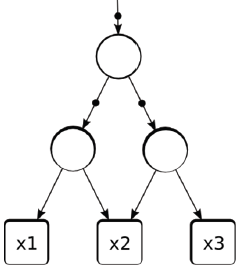
\includegraphics{images/AIG.png}
	\caption{An And-Inverter Graph representing the Boolean formula $\phi = (x_1 \wedge x_2) \vee (x_2 \wedge x_3)$}
	\end{center}
\end{figure}



\section{MaxSAT}
A subclass of SAT problems is called \textbf{weighted maximum satisfiability}, or \textbf{MaxSAT}. A MaxSAT formula can be seen as optimization extension of SAT: the formula is defined as a conjunction of clauses and, for each clause, a weight (a positive real number) is assigned. Given a Boolean assignment of its variables, a score is calculated considering the weights of all satisfied clauses. This addition changes the perspective of the problem: every assignment can now be considered acceptable, since some clauses can be falsified. As a consequence MaxSat defines a new task: find a Boolean assignment so that the associated score is maximum. Similarly to SAT, multiple assignments can be the solution of a MaxSAT instance, resulting in multiple valid assignments. \\
To better understand it, we cover it using an example. We will consider the following Boolean formula:

\begin{equation}
    \varphi = ( x_1 \vee x_2) \wedge (\neg x_1 \vee \neg x_2) \wedge ( x_1 \vee \neg x_2) \wedge (\neg x_1 \vee x_2)
\end{equation}

Each clause has also an additional weight: first clause from left has a score of 1, each subsequent clause's weight is higher by 1 with respect to the precedent. Clearly no assignment could satisfy all clauses at the same time, but this has no interest since we are solving a MaxSAT problem. Quickly considering all possible assignments, we can state that the one guaranteeing the maximum total score is $x_1 = \bot$ and $x_2 = \bot$, satisfying respectively the clauses with weights 2, 3 and 4. No other Boolean assignment could achieve the same result, so this is the only solution to our MaxSAT problem.

\section{Satisfiability Modulo Theories}

Satisfiability Modulo Theories represents an extension to the SAT problem. The input and the final goal remain the same as SAT: this means that we have to deal with first-order logic formulas and we search for a valid assignment of variables satisfying such formulas. The main difference relies on the fact that binary boolean variables can be replaced by predicates and functions belonging to non-binary theories. Some of the most relevant theories in the Formal Verification fields are:

\begin{itemize}
    \item Linear Arithmetic over Integers, Real or both (LIRA)
    \item Bit vector arithmetic (BV)
    \item Floating-point arithmetic(FP)
    \item Uninterpreted functions (UF)
\end{itemize}

Given the non-binary nature of these theories, novel approaches have been studied and tested to efficiently evaluate the satisfiability of a given formula. At the current state, the most widely used algorithm is known as \textbf{Lazy SMT solving}\cite{lazysmt}, whose core idea will be briefly explained to the reader for a better comprehension. Given an SMT formula and a subset of theories, we produce a Boolean abstraction formula in which each non-binary predicate is replaced by a binary variable. This new formula is then fed to a CDCL SAT solver and used to search a satisfiable assignment. When a satisfiable assignment is obtained, the corresponding set of T-literals that make up the original problem are fed to specialized theory solvers. If each clause if T-consistent, then we proved the satisfibility of the original formula; otherwise, the conflict clauses causing unsatisfiability are extracted and learned by the CDCL algorithm , permitting the evaluation of new assignments. The algorithm goes on until satisfiability is proved or no more assignment can be returned, proving its unsatisfiability. \\
In order to be evaluated, the instance of a SMT problem has to be instantiated using a standard format. Regarding SMT encoding, SMT-LIB is the international initiative on top of which most SMT solvers are built. SMT-LIB does not only promote common input and output languages for SMT solvers; it also provides standard rigorous descriptions of background theories used in SMT systems and establishes benchmarks that can be used to test the solvers to highlight weaknesses and strengths. \\
The syntax of SMT-LIB-based tools is quite simple. First, we define properties of the problem and solver options (for instance determine if we want to extract unsat cores). We can also set a theory, so that efficient algorithms and heuristics are applied during execution to improve performances. After this introduction, we declare constants, variables and functions. Then assertions are expressed: they bind the values of variables, restricting the range of satisfying solutions. A simple example is provided in listing 2.1. \\
\begin{lstlisting}[style=interfaces,caption=An example of SMT-LIB encoding.]
(set-info :smt-lib-version 2.6)
(set-option :print-success false)
(set-option :produce-models true)

(declare-const x Int)
(declare-const y Int)
(declare-fun f (Int) Int)

(assert (= (f x) (f y)))
(assert (not (= x y)))

(check-sat)
(get-value (x y))
\end{lstlisting}
Among the solvers accepting SMT-LIB as input format, University of Trento and the Bruno Kessler Foundation have developed a SMT solver, called MathSAT. The code, written in C++, support all the theories mentioned above, plus other logics as Arrays arithmetic. It also supports interesting functionalities such as generation of models and proofs for satisfiable problem, extraction of unsatisfiable cores for the unsatisfiable ones and incrementality.

\section{Optimization Modulo Theories}

Optimization Modulo Theories represents an extension to the SMT framework. In addition to the already described first-order formulas involving non-binary logics, we focus on defining one or more non-binary objective function. As a result, retrieving a satisfying assignment is not sufficient anymore: the goal is now obtaining a valid model while minimizing/maximizing the objective functions, according to our choice.\\
The language used to encode OMT problems is an extension of the SMT-LIB standards. In addition to the syntax already discussed for SMT-LIB, some commands are available to define the cost functions we desire to optimize and the direction of optimization. The structure of this command is:

\begin{equation*}
    \textbf{solve [maximize/minimize] $<$cost function$>$}
\end{equation*}

If permitted by the solver, we can also write multi-objective optimization problems. multi-objective optimization problems  require the presence of some instructions to determine the philosophy adopted to determine the goodness of a solution. Example of valid approaches are:

\begin{itemize}
    \item \textbf{Pareto Optimality}: given two different solutions and a set of $n$ cost functions $x_1...x_n$, we state that the first solution is better to the second one according to this criterion if there exists a cost function $x_i$ (where $1\leq i\leq n$) so that $x_i$ calculated on the values of the first solution dominates the value obtained using the second solution; in addition to that, for each cost function $x_i$ the first solution obtain better or equal values than the second one. When using this criterion, multiple solutions can satisfy these conditions: the set of these valid assignment is called \textbf{Pareto front}.
    \item \textbf{Lexicographic Optimality}: first we define a total order among the various cost functions, determining  a hierarchy. Given two different solutions, we will first compare the value of the first cost function on this hierarchy for both of them; if one of these solutions dominates the other it is chosen as optimal, otherwise we will compare the value associated to the second cost function and so on until reaching the last one.
\end{itemize}

The jointly work between FBK and University of Trento gave birth to an Optimization Modulo Theories solver, \textit{OptiMathSAT} \cite{pa25}*.

\section{Constraint Programming and MiniZinc}

Constraint Programming is an alternative paradigm for solving combinatorial problems. A Constraint Satisfaction Problem (CSP) is defined by a set of variables, each one with its domain of values, and a number of constraints, relations among a subset of the variables. A simple example of constraint is called ALLDIFFERENT: given some variables as input to this relation, it ensure no involved variable will assume the same value. The usual output of a CSP is a a valid assignment for each declared variables, if possible. The CSP has been extended to deal with the search of optimal solution with respect to some objective function, similarly to what happened to SMT: these problem are referred as Constraint Optimization Problems (COP).
Due to the large amount of constraint available and its representational power, Constraint Programming popularity is growing in the last years and it is actually used in some formal verification related tasks. \\
MiniZinc is the most popular high-level declarative language used to encode both CSP and COP instances. It is developed at Monash University in collaboration with Data61 Decision Sciences and the University of Melbourne. Each MiniZinc model first declares each variable needed to define the problem; optionally a value can be assigned, obtaining a parameter whose behaviour is similar to constants. Variables which are not initialized are known as decision variable and their value is determined by the solver, trying to satisfying the conditions that will follow. The next component of the model are the constraints, Boolean expression defining bounds to the value each decision variable can assume. Lastly we have a line expressing if we are working with CSP (so we only focus on knowing if there exists an assignment satisfying each variable domain and making true all constrains) or COP (in this case the user has to define the objective function to optimize and the direction of optimization). A simple example is provided in listing 1.2.

\begin{lstlisting}[style=interfaces,caption=An example of MiniZinc encoding regarding the popular Stable Marriage Problem.]
int: n;
enum Man = anon_enum(n);
enum Woman = anon_enum(n);
array[Woman, Man] of int: rankWomen;
array[Man, Woman] of int: rankMen;
array[Man] of var Woman: wife;
array[Woman] of var Man: husband;

constraint forall (m in Man) (husband[wife[m]]=m);
constraint forall (w in Woman) (wife[husband[w]]=w);
constraint forall (m in Man, o in Woman) (
     rankMen[m,o] < rankMen[m,wife[m]] -> 
         rankWomen[o,husband[o]] < rankWomen[o,m] );
constraint forall (w in Woman, o in Man) (
     rankWomen[w,o] < rankWomen[w,husband[w]] -> 
         rankMen[o,wife[o]] < rankMen[o,w] );
solve satisfy;
\end{lstlisting}

\subsection{Bridging CP and OMT}

OMT presents some specific affinities that make it a valid candidate to deal with CSP: the availability of decision procedures for infinite-precision arithmetic, the efficient combination of
Boolean and arithmetical reasoning and the ability to produce conflict explanations are shared between the two paradigms and it is not a case both are used to deal with formal verification problems. Achieving this task benefits the progression of the current state-of-the-art: the comparison between OMT solvers and CP tools on problems that do not belong to their original application domain extends their application in novel fields and speed up the process of finding critical points for future research. \\ 
Despite that, transforming a CP instance into a OMT problem is not trivial; in particular there are multiple valid formulation of a CP problem into an OMT instance. Using one option instead of the others requires particular attention, since this choice could drastically affect performances (as shown in []). This situation represents the first issue hardening the bridging task. In addition to this difficulty, there are some MiniZinc features that requires a careful mapping to the SMT-LIB standard. In particular:

\begin{itemize}
    \item FlatZinc support three basic scalar types (int, float and bool) and two compound types (set and array). Compound types do not have a direct correspondence in the SMT-LIB standard; moreover integer and float can be represented using finite precision (using respectively bit-vector and floating point arithmetic) or applying the linear arithmetic theory.
    \item MiniZinc introduced local and global constraints to express complex relations among variables. OMT solver currently do not introduce ad hoc decision procedures to manage them efficiently.
    \item MiniZinc is capable of dealing with non-linear and transcendental functions, such as the logarithm or the cosine function. On the other hand, not every solver built on SMT-LIB support them.
\end{itemize}

\section{Quantum Annealer}
\label{sec:quantum}

In order to achieve efficiency in solving the hardest tasks, one of the proposed techniques involves the exploit of quantum technologies. In the case at issue \textbf{Quantum Annealers (QA)} have been proved to be effective for this task. \\
Quantum annealers are specialized chips that exploit particular quantum effects (such as superposition and tunneling) to sample or minimize energy configurations. Each configuration is composed by binary variables $z_i$ which can assume a value -1 or 1, representing their state. The energy configuration can be represented using the Ising Hamiltonian function, whose structure is the following:

\begin{equation}
    H(\textbf{\underline{z}}) = \sum_{i \in V} h_iz_i + \sum_{\langle i,j\rangle \in E} J_{ij} z_iz_j
\end{equation}

Formula 2.7 shows the parameters that influence the system's behaviour: 

\begin{itemize}
    \item $h_i$ are called \textbf{biases} and are defined as a real number in range $[-2,2]$
    \item $J_{ij}$ and lastly $J_{ij}$ are called \textbf{couplings} to the connected pair of qubits at index $i$ and $j$ and is a real number in range $[-1,1]$.
\end{itemize}

The search of the ground state of an Ising model is known as \textbf{quadratic unconstrained binary optimization (QUBO)} problem. \\

\subsection{The SQUID transistor}

 The minimal unit composing a quantum annealear is called \textbf{qubit}: a qubit can assume a symbol value of 0, 1 or a superimposition of 0 and 1. The physical devices used to build qubits are the \textbf{Superconducting QUantum Interference Devices (SQUID)}, where the word interference refers to the electrons patterns that give birth to quantum effects. The structure of this qubit transistor is defined by two superconductor coupled by a weak link, usually a thin insulating barrier. Transistors satisfying these conditions are subject to the \textbf{Josephson effect}. The superconducting qubit structure instead encodes 2 states as tiny magnetic fields, which either point up or down. We call these states +1 and -1, and they correspond to the two states that the qubit can 'choose' between. Using the quantum mechanics that is accessible with these structures, we can control this object so that we can put the qubit into a superposition of these two states as described earlier. So by adjusting a control knob on the quantum computer, you can put all the qubits into a superposition state where it hasn't yet decided which of those +1, -1 states to be.\\
  Each ring can be superimposed to other rings, defining more complex architectures and admitting an exchange of information among different qubits (thus the definition of couplings in the Ising formula). Figure 2.2 shows the physical structure of a qubit.\\
  
  \begin{figure}[t]
	\begin{center}
	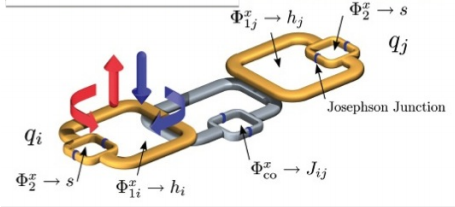
\includegraphics{images/QA.PNG}
	\caption{A physical representation of qubits in an Quantum Annealer.}
	\end{center}
\end{figure}

\subsection{D-Wave Quantum Annealers}

The entire energy configuration can be represented as a connected graph, where vertexes represent our qubits and edges represent connections between qubits. This configuration highlights how qubits' ground state is not considered independently, but their interaction with neighbour qubits alters the final energy state of our configuration. The choice of a specific quantum annealer influences the formulation of an Ising model: each annealer has a specific architecture and specific properties, constraining the formulation of a problem. In this thesis we will concentrate on annealers developed by the Canadian company D-Wave \cite{Dwave}. In the beginning, the Canadian company aimed in increasing the number of available qubits, obtaining Moore-like growth as shown in figure 2.3. 
\begin{figure}[t]
	\begin{center}
	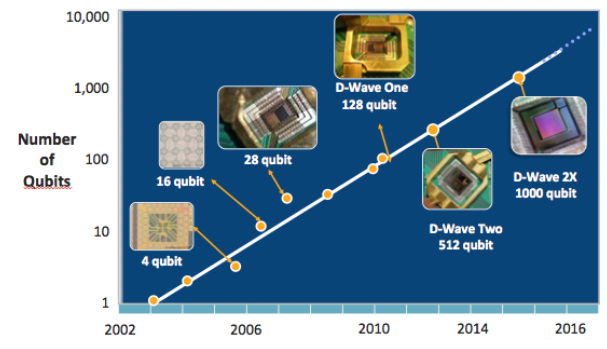
\includegraphics{images/DwaveMoore.PNG}
	\caption{D-Wave annealers growth over the years. Courtesy of D-Wave Systems Inc.}
	\end{center}
\end{figure}
In a second phase, the company put its effort in defining novel structures with better connections and fewer wasted qubits. Currently D-Wave has already developed and produced a first quantum system, known as \textbf{Chimera}. The basic features of this architecture are:

\begin{itemize}
    \item The basic unit is the tile, which contains 8 qubits.
    \item Qubits of a cell unit are grouped into two groups (the horizontal and vertical qubits): qubits belonging to the same group are connected to qubits of the opposite group thanks to couplings.
    \item Unit cells are tiled vertically and horizontally with adjacent qubits connected, creating a 16 $\times$ 16 lattice of 2048 qubits.
    \item From previous constraints, we can see how each qubits can be connected to a maximum of 6 other variables, resulting in the sparsity of the adjacency matrix. Qubits that are not connected to each other are managed setting the related coupling value to 0.
\end{itemize}

In addition to this structure, D-Wave is already studying new architectures overcoming the sparsity of the graph and the absence of cliques; in 2019 the company proposed a new architecture called \textbf{Pegasus}. The properties of this system are:

\begin{itemize}
    \item The number of qubits is $24*N*(N-1)$, where $N$ is an integer number.
    \item The architecture is less modular than Chimera and, in particular, it is not structured in 8-qubit tiles.
    \item Pegasus graph is less sparse than Chimera, presenting an higher number of interleavings among qubits (exactly 15 couplings for a single qubit).
    \item The increasing number of couplings have given the opportunity to obtain huge progress with respect to the old model. In particular, Pegasus provides 3 and 4-cliques and qubit duplication.
\end{itemize}

Figure 2.4 shows the graphs representing both Chimera and Pegasus topologies, rapidly displaying the main differences between the two models. 

\begin{figure}
\centering
\begin{subfigure}[b]{0.55\textwidth}
   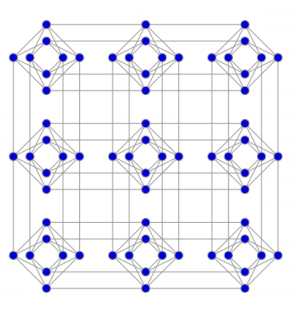
\includegraphics[width=1\linewidth]{images/QATile.PNG}
   \caption{}
   \label{fig:Ng1} 
\end{subfigure}

\begin{subfigure}[b]{0.55\textwidth}
   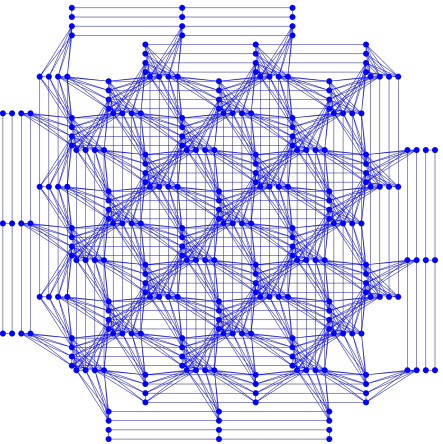
\includegraphics[width=1\linewidth]{images/Pegas.PNG}
   \caption{}
   \label{fig:Ng2}
\end{subfigure}
\caption{A representation of the two architecture proposed by D-Wave, respectively: (a) $3*3$ tiles sub-graph of Chimera (b) the graph of Pegasus6.}
\end{figure}

\newpage


      \chapter{Related work}
\label{cha:related}

In this chapter will deepen on the SAT-to-Ising reduction problem, which has been proved to be useful when trying to exploit properties of quantum computing to reduce the computation time to solve SAT problems. We will discuss a preliminary algorithm that have been studied at University of Trento, distinguishing the procedure adopted to encode simple formulas from complex Boolean instances.

\section{SAT-to-Ising}
\label{sec:SATtoQUBO}

As already stated in the previous paragraphs, SAT main issue is the exponential growth of complexity, stopping computer scientists in investigating hard tasks involving a small number of variables. Quantum computing, on the other hand, exploit specific phenomena such as tunneling to search the minimum of an Ising problem, optimizing computational time. If we would be able to encode SAT/MaxSAT problem into an Ising Hamiltonian problem, we could exploit quantum calculus properties to verify satisfiability of out original problems, drastically reducing computational time. The task described is known as \textbf{SAT-to-QUBO}. \\
Computer scientists use Quantum Annealers as black-box algorithms which are fed to QUBO problems, whose formulation is similar but not identical to an Ising problem:

\begin{equation}
    H(\textbf{\underline{z}}) =\theta + \sum_{i \in V} h_iz_i + \sum_{\langle i,j\rangle \in E} J_{ij} z_iz_j
\end{equation}

As we can see qubits, biases and couplings are present in our formulation; in addition to them we consider the parameter $\theta_0$, which is called offset and falls into the range $(+\infty, -\infty)$. \\
Given a SAT problem, we are interested in finding a variable placement \textbf{x} $\rightarrow$ \textbf{z} on the quantum annealer qubits and the values of offset, biases and couplings so that:

\begin{equation}
    P_F(\underline{\textbf{x}} | \underline{\theta}) = 
    \left\{
        \begin{array}{lr}
            = 0, & if \textbf{ \underline{x}} \models F \\
            \geq g_{min}, & if \textbf{ \underline{x}} \models T
        \end{array}
    \right\}
\end{equation}

The gap $g_{min}$ is essential to manage sensitivity of the quantum annealer: the optimization will be affected by noise generated by the non-zero Kelvin temperature and , so it will be rarely the case that not satisfying assignment will get 0 as final score. Setting the gap (and trying to find the highest gap possible satisfying the problem) will help us in discriminating acceptable assignments and not acceptable ones.
For instance, a formula we can easily encode into an Ising Hamiltonian function is $\varphi = x_1 \iff x_2$. A simple penalty function would be $P_F(\underline{\textbf{x}} | \underline{\theta}) = 1 - x_1x_2$, whose gap for satisfying assignment is 2. \\
The current formulation of our problem presents some issues:

\begin{itemize}
    \item Chimera tile architecture is quite limited: the absence of clique and the sparsity of the matrix reduce the number of problem we can represent.
    \item The problem is actually overconstrained: you need to search your solution checking O($2^{|\textbf{\underline{x}}|}$) models/countermodels. You have also to deal with the degrees of freedom of its formulation caused by biases and couplings.
\end{itemize}

To overcome this difficulties, we can add a non-fixed numbers of ancillary variables to provide the missing links. The problem will slightly change into the task:

\begin{equation}
    min_{[\textbf{\underline{a}} \in \{-1,1\}^k]} P_F(\underline{\textbf{x}},\underline{\textbf{a}} | \underline{\theta}) = 
    \left\{
        \begin{array}{lr}
            = 0, & if \textbf{ \underline{x}} \models F \\
            \geq g_{min}, & if \textbf{ \underline{x}} \models T
        \end{array}
    \right\}
\end{equation}

The more ancillary variables we add to our formulation, the more complex the resulting task will be, so we will always try to limit their use only when necessary. Ancillary variable are essential for basic encoding formulas: an example could be $\varphi = x_3 \iff (x_1 \vee x_2)$. If the Quantum Annealer admitted cliques the encoding would be trivial; since this is not the case, an ancilla is added to obtain a valid penalty function:

\begin{equation}
    P_F(\underline{\textbf{x}},\underline{\textbf{a}} | \underline{\theta}) = \frac{5}{2} - \frac{1}{2} x_1 - \frac{1}{2} x_2 + x_3 + \frac{1}{2} x_1x_2 - x_1x_3 - x_2a -x_3a
\end{equation}

Figure 1.3 shows the positioning of the obtained Ising Hamiltonian functions into a Chimera tile.
\begin{figure}[t]
	\begin{center}
	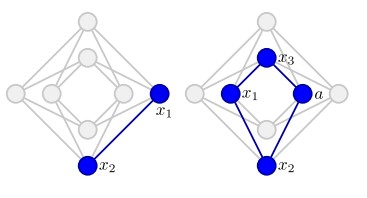
\includegraphics[width=.7\textwidth]{images/Ising1+2.png}
	\caption{On the left, a valid positioning of qubits into a Chimera tile for the formula $\varphi = x_1 \iff x_2$. On the right, a valid positioning for the formula $\varphi ' = x_3 \iff (x_1 \vee x_2)$. Both architectures are inspired by the penalty functions discussed in this paragraph.}
	\end{center}
\end{figure}

\subsection{Determining the penalty function}

The task of retrieving the parameters characterizing the penalty function of a Boolean formula can be espressed by a SMT problem:

\begin{equation}
    \forall \textbf{\underline{x}} \left[
        \begin{array}{lr}
            ( F(\underline{\textbf{x}}) \rightarrow \forall \underline{\textbf{a}}.(P_F(\underline{\textbf{x}},\underline{\textbf{a}} | \underline{\theta}) \geq 0 )) \land \\
            ( F(\underline{\textbf{x}}) \rightarrow \exists \underline{\textbf{a}}.(P_F(\underline{\textbf{x}},\underline{\textbf{a}} | \underline{\theta}) = 0 )) \land \\
            ( \neg F(\underline{\textbf{x}}) \rightarrow \forall \underline{\textbf{a}}.(P_F(\underline{\textbf{x}},\underline{\textbf{a}} | \underline{\theta}) \geq g_min )) \land \\
            ( \neg F(\underline{\textbf{x}}) \rightarrow \exists \underline{\textbf{a}}.(P_F(\underline{\textbf{x}},\underline{\textbf{a}} | \underline{\theta}) = g_min )) \land \\
        \end{array}
    \right]
\end{equation}

The last row of equation (2.2) can be omitted if we are not searching an exact penalty function. Since this omission drastically reduce the computational time to search a valid solution, we will usually consider it omitted. \\
Classic satisfiability theories do not deal with quantifiers, so it is essential to successfully remove them, obtaining and equivalent formula. The most popular approach adopted is \textbf{Shannon expansion}. Given an universal quantifier with respect to a set of variables, we can build an equivalent formula as the union of set of clauses whose structure is identical to the original structure, additionally setting the variables inside the considered set to one of their possible value. On the other hand, if we are presented an existential quantifier, we can recycle the previous algorithm but we will connect all the clauses using the AND operator instead of OR. Clearly the procedure is exponential (the more variables we consider, the more combinations of true/false value we can obtain). Once the expansion takes place, the original problem is reduced to the following SMT problem on linear real algebric theory:

\begin{equation}
    \Phi(\theta) =
        \begin{array}{lr}
            \bigwedge_{Z_i\in\textbf{\underline{x}},\textbf{\underline{a}}}(-2\leq\theta_i) \land (\theta_i\leq 2) \\
            \land\  \bigwedge_{Z_i,Z_j\in\textbf{\underline{x}},\textbf{\underline{a}}, i<j}(-1\leq\theta_{ij}) \land (\theta_{ij}\leq 1) \\
            \land\ \bigwedge_{\{\textbf{\underline{x}}\in\{-1,1\}^n|F(\textbf{\underline{x}}=\top\}} \bigwedge_{\textbf{\underline{a}}\in\{-1,1\}^h}P_F(\underline{\textbf{x}},\underline{\textbf{a}} | \underline{\theta}) \geq 0 \\
            \land\ \bigwedge_{\{\textbf{\underline{x}}\in\{-1,1\}^n|F(\textbf{\underline{x}}=\top\}} \bigvee_{\textbf{\underline{a}}\in\{-1,1\}^h}P_F(\underline{\textbf{x}},\underline{\textbf{a}} | \underline{\theta}) = 0 \\
            \land\ \bigwedge_{\{\textbf{\underline{x}}\in\{-1,1\}^n|F(\textbf{\underline{x}}=\bot\}} \bigwedge_{\textbf{\underline{a}}\in\{-1,1\}^h}P_F(\underline{\textbf{x}},\underline{\textbf{a}} | \underline{\theta}) \geq g_{min} \\
            \land\ \bigwedge_{\{\textbf{\underline{x}}\in\{-1,1\}^n|F(\textbf{\underline{x}}=\top\}} \bigvee_{\textbf{\underline{a}}\in\{-1,1\}^h}P_F(\underline{\textbf{x}},\underline{\textbf{a}} | \underline{\theta}) = g_{min} \\
        \end{array}
\end{equation}

While the SMT formulation will help us in determining if there exists a valid assignment of parameters to apply the SAT-to-Ising conversion, we recall from paragraph 2.1 that determining the highest value that $g_{min}$ can assume is a fundamental task; as a consequence, we can use equation 2.6 to define an OMT problem, where the cost function is simply $g_min$ and the direction of optimization is the search of the maximal.

\section{Issues in Encoding for Quantum Annealers}

Converting a Boolean circuit into a QUBO formulation would apparently seem an easy task to achieve: actually the nature and the architecture of the annealers drastically reduce the number of SAT problems we can embed. The main issues causing the inefficiency are:

\begin{itemize}
    \item \textbf{The number of qubits is not unlimited}: even though the recent architectures provides more than 2000 qubits, they are usually not enough to encode the majority of circuits.
    This is due by the nature of the two encoding: the number of qubits representing the input width and the circuit size are two different metrics for complexity, where the former is definitively bigger than the latter. 
    \item \textbf{The number of couplings is not unlimited}: as already mentioned in paragraph, each architecture can be interconnected to a limited number of other qubits. Consequently, the encoding process has to take into account this upper limit and, if more connections are required, map a Boolean variable into multiple qubits.
    \item \textbf{Noise impacts the system performance}: the ideal condition of a quantum annealer would require a temperature of 0 K and to be heavily shielded by electro-magnetic rays, preserving the properties of the superconductor rings. In reality these conditions are never met and D-Wave system are subject to performance degradation.
\end{itemize}

Because of the problems described above, advanced algorithms have been studied and tested in order to reduce the amount of qubits required during the reduction of the SAT circuit.

\section{Encoding complex Boolean formulas}

Determine an efficient encoding is decisive, given the limited of number of qubits of Chimera. Penalty functions have some properties we can exploit to iteratively build complex formula from easier ones. The first property is \textbf{NPN-Equivalence}: given a boolean formula $F(\textbf{\underline{x}})$ with its associated penalty function $P_F(\underline{\textbf{x}},\underline{\textbf{a}} | \underline{\theta})$ and a new Boolean function $F^*(\textbf{\underline{x}})$ identical to the previous one but a single variable at a generic index $i$ (so that it appears with inverse cardinality in the new formulation), we can recycle $P_F(\underline{\textbf{x}},\underline{\textbf{a}} | \underline{\theta})$ to obtain the penalty function for the new problem. In particular, $P_{F^*}(\underline{\textbf{x}},\underline{\textbf{a}} | \underline{\theta}) = P_F(\underline{\textbf{x}},\underline{\textbf{a}} | \underline{\theta}^*)$ where $\theta^*$ is a new vector of biases and couplings so that for each $z,z'\in \textbf{\underline{x}},\textbf{\underline{a}}$: \\ \\ \\

\begin{equation}
    \theta_z^* = 
    \left\{
        \begin{array}{lr}
            -\theta_z, & \textit{if }z = x_i \\
            \theta_z, & otherwise
        \end{array}
    \right\}
\end{equation}

\begin{equation}
    \theta_{zz'} = 
    \left\{
        \begin{array}{lr}
            -\theta_{zz'}, & \textit{if }z = x_i \vee z' = x_i\\
            \theta_{zz'}, & otherwise
        \end{array}
    \right\}
\end{equation}


So once we extract the penalty function for a Boolean Formula, its variants can be easily computed switching signs of biases and coupling. For instance, if we had the Boolean formula $\varphi = x_1 \iff -x_2$, we could easily invert signs of couplings and biases associated with $x_2$, trivially obtaining $P_F(\underline{\textbf{x}} | \underline{\theta}) = 1 + x_1x_2$. \\
The second property fundamental to simplify the task of retrieving penalty functions is the \textbf{AND-decomposition}. Given a Boolean function that can be rewritten as a combination of simpler functions so that $F(x) = \land_k F_k(\underline{x}^k)$, where each $F_k(x)$ is associated to a penalty function $P_{F_k}(\underline{x^k},\underline{a^k}|\underline{\theta^k})$ with minimum gap $g^k_{min}$, $\underline{x} = \cup_k \underline{x^k}$ and $\underline{a} = \cup_k \underline{a^k}$, then we can define a penalty function for the original formula in the following way:

\begin{equation*}
    P_{F}(\underline{x},\underline{a}|\underline{\theta}) = \sum_k P_{F_k}(\underline{x^k},\underline{a^k}|\underline{\theta^k}) \; \textrm{        with        } g_{min} = \min_k(g^k_{min})
\end{equation*}
\begin{equation}
    \theta_i = \sum_k \theta^k_i
\end{equation}
\begin{equation*}
    \theta_{ij} = \sum_k \theta^k_{ij}
\end{equation*}

Equation 2.8 works in the case each bias and coupler value satisfies its range. The subformulas making up the decomposition could share some common variables and, in some cases, this could lead to the attainment of out-of-range biases and couplers. This issue can be easily fixed: we can scale up or down the impact of each penalty function adding a weight $w_k$ greater than 0. This addition slightly modifies equation 2.8, determining the general formulation:

\begin{equation*}
    P_{F}(\underline{x},\underline{a}|\underline{\theta}) = \sum_k P_{F_k}(\underline{x^k},\underline{a^k}|\underline{\theta^k})*w_k \; \textrm{        with        } g_{min} = \min_k(g^k_{min})*w_k
\end{equation*}
\begin{equation}
    \theta_i = \sum_k \theta^k_i*w_k
\end{equation}
\begin{equation*}
    \theta_{ij} = \sum_k \theta^k_{ij}*w_k
\end{equation*}

Adding these weights weakens the minimum gap, so it is not used in practice. An alternative to equation 2.9 relies on the renaming of the shared variable, so that each $\underline{x}^k$ is disjoint with respect to the others. To achieve this goal, when two conjuncts $F_k, F'_k$ share a Boolean variable $x_i$ we rename the second occurrence with a fresh variable $x'_i$ and conjoin the two variable using the simple formula $(x_i \iff x'_i)$. Now we can re-define the original formula and its associated penalty function as:

\begin{equation*}
    F^*(\underline{x}^*) = \bigwedge_k F_k(\underline{x}^{k*}) \land \bigwedge_{\{ x_i \textrm{  shared}\}} (x_i \iff x'_i) 
\end{equation*}
\begin{equation}
    P_{F^*}(\underline{x}^*,\underline{a}|\underline{\theta}) = \sum_k P_{F_k}(\underline{x^k},\underline{a^k}|\underline{\theta^k}) + \sum_{\{ x_i \textrm{  shared}\}} (1 - x_ix'_i)
\end{equation}
\begin{equation*}
    g_{min} = min_k(g^k_{min},2)
\end{equation*}

Given the nature of the penalty functions for $(x_i \iff x'_i)$, whose gap is 2, we ensure no issue can emerge and no parameter range error can be observed.
Combining the two properties above we can define the procedure to apply to retrieve penalty functions decomposing Boolean formulas into smaller chunks, easier to convert:

\begin{itemize}
    \item First we Tseitin-style decompose $F(x)$ into an equi-satisfiable formula so that:
    
    \begin{equation}
        F*(\underline{x},\underline{y}) = \bigwedge^{m-1}_{i=1} 
        (y_i \iff F(\underline{x}^i,\underline{y}^i)) \wedge F_m(\underline{x}^m,\underline{y}^m)
    \end{equation}
    
    \item When two conjuncts $F_1$ and $F_2$ share one variable $y_j$, rename the second with a fresh new variable $y_i'$, conjoining $(y_i' \iff y_j)$.
    \item Compute the penalty function for each conjunct separately.
    \item Sum the penalty functions obtained in the previous step to obtain a single function. 
\end{itemize}

From the algorithm described above, we can define a universal approach to deal with larger Boolean functions, avoiding the application of the SMT formulation which results too much time and resource demanding. \\
Before starting the encoding, we compute in advance a collection of valid encoding for simple SAT formulas so that they can be mapped using a low number of qubits (in particular when using the Chimera architecture we aim to encode the formula using a single tile). The original SAT formula we want to encode is pre-processed, in order to reduce its size or complexity in terms of its graphical
representation. As an example, a good pre-processing approach is using the and-inverted-graph representation, which transform a formula in a combination of AND and NOT functions. Using the simplified structure and the previously computed library we then define a mapping between Boolean variables and the annealer's qubits. This phase represents the most complex and resource-demanding procedure of the algorithm. The fundamental steps of this procedure are:

\begin{figure}[t]
	\begin{center}
	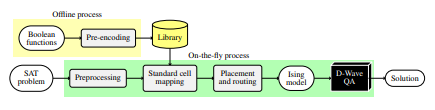
\includegraphics[width=\textwidth]{images/LargeBool.PNG}
	\caption{A graphical representation of the encoding process for larger Boolean functions.}
	\end{center}
\end{figure}

\begin{itemize}
    \item Use the library of pre-computed penalty functions to map each function part of the decomposed and simplified SAT formula into a valid QUBO encoding. This phase is known as standard cell mapping.
    \item Now it is necessary to embed the entire formula onto the QA hardware. To achieve this task, we first assign a disjoint subgraph of the QA hardware graph to each penalty function chosen in the previous step.
    \item Lastly we need to ensure that qubits representing the same variable are chained so that they can assume the same value when given as input to the annealer: we can accomplish it using penalty functions in the form $1 - x_1x_2$, where $x_1$ and $x_2$ are qubits representing the same variable. This step is a direct consequence to formula 2.8.
\end{itemize}

The algorithm is heavily discussed in \cite{varotti} and more details are provided about the choice of and the heuristic adopted to obtain a more stable encoding, but for the sake of brevity we will not discuss it further. Figure 2.4 summarizes the entire process.

\pagebreak
      
\vspace*{\fill}
\begin{center}
   \Huge{\textbf{Part II}} \\
   \Huge{\textbf{Contributions}}
\end{center}
\vspace*{\fill}

\newpage
      \chapter{Tool analysis}
\label{cha:analysis}

In this chapter we will discuss the state-of-the-art tool developed by the jointly work of University of Trento and D-Wave. More specifically we will emphasise critical points of the current version, suggesting possible direction to improve the performance of the algorithm.

\section{The issue of co-tunnelling}

The major issue while converting a SAT problem into a Ising instance is represented by the problem known as \textbf{co-tunneling}. Co-tunneling is a side-effect issue caused by the presence of long chains of qubits in the annealer's placement \cite{cotunneling}. [Discuss cotunneling in more details]

\section{Studying the Ising encoding}

To determine the behaviour of the placement algorithm and to easily understand how frequently long chains are generated, it was required to graphically represent the annealer architecture when applied to a SAT-to-Ising encoding task. \\
A new script has been developed to accomplish this task, called \textit{graph\_to\_dot}. The first step was the building of a graph reflecting the architecture of the quantum annealer chosen at execution. Information about the topology of the network has been retrieved using \textbf{D-Wave NetworkX}, an extension of NetworkX providing tools and data for working with the D-Wave systems \cite{dwavenetx}. Data about the has been collected from the \textit{place\_and\_route} algorithm: for each AIG-related subformula the algorithm returns a subset of qubits to the graph and the values of weights extracted from the pre-computed libraries. Using this information, we choose a color for each penalty function and use it to determine the related qubits and the involved couplings in the graphical representation. The color of edges representing chains of a Boolean variable have been set to black. 
An example of Boolean formula placement is shown in figure xx.

\begin{figure}[]
	\begin{center}
	\includegraphics[width=0.8\textwidth]{images/graph7.png}
	\caption{A graphical representation of the encoding of a benchmark problem, C17, into the Pegasus architecture.}
	\end{center}
\end{figure}

The major issue visible from the figure is the presence of long chains of qubits. As already stated in paragraph 3.1, higher size of chains worsen the stability of the annealers in the search of the Hamiltonian final state. Each qubit belonging to the chain can be potentially more useful: unused arcs adjacent to them and set to 0 could be used to determine novel penalty functions. The results would be more complex structures that could help us in obtaining better penalty function, less prone to be subject to co-tunelling and with higher $gap_{min}$.
The script was integrated to the original code as a debug option, permitting other users to test their encoding and better understanding the results behind the implemented procedures.

\section{The searchPF function}

The previous section suggested the idea to recompute penalties function reducing the length of the chains. These nodes, used as ancillas and considering their unused couplings, could provide more complex encoding, reducing the co-tunneling effect and guaranteeing more energy stability. The tool already provide a class of algorithms to compute offset, biases and couplings of an Ising problem, given a topology and the Boolean function. Each function provided some specific constraints in order to satisfying properties such as getting the maximum $g_{min}$  The function relevant to the scope of this thesis, called \textbf{searchPF}, was the most suitable to our purpose, given its simplicity and its ease to be extended. \\
\textit{SearchPf} requires as input the following objects:

\begin{itemize}
    \item A graph representing the topology of the involved qubits. Graphs are created using the \textit{GraphViz} library, setting the nodes name as the integer in the range [1,$N$] with N the number of qubits.
    \item A function representing the Booolean formula we desire to map into the given graph.
    \item Two integers $nx$ ans $na$, representing respectively the number of qubits representing the variables and the number of qubits working as ancillas.
\end{itemize}

In order to get the weights defining the penalty function, an Optimization Satisfiability problem is instantiated using the previously mentioned parameters. The problem is fed to OptiMathSAT, which returns in response an empty if no valid penalty functions has been found; otherwise, a dictionary containing the parameters value and the minimum gap is returned. Multiple constraints are set to map the problem into the SMT-LIB language:
 
\begin{itemize}
    \item \textbf{Architecture constraints}: we ensure the resulting penalty function respects the topology of the given graph. As a consequence, some couplings need to be set to 0 a.
    \item \textbf{Range constraints}: As stated in section 1.5, values of biases and couplings need to be constrained so that they cannot violate their ranges. For each coupling and each bias an assert condition setting lower an upper bounds are added to the OMT encoding.
    \item \textbf{Expansion gap constraints}: in order to retrieve the parameters of the Ising function we have to solve the  quantified OMT problem described in 
\end{itemize}

The function has been heavily tested to learn its behaviour, its complexity and thus offering cues for improvements. First we studied the relation between the required time to obtain a solution to the OMT problem and the number involved variables, with the goal of determining an upper bound for the number of nodes so that the OMT problems can return their solution in a feasible amount of time to be applied in real-life applications. Table 3.1 shows the results of this analysis; we can see how we are bound to use a very low number of qubits.
\begin{table}[]
\centering
\begin{tabular}{|c|c|}
\hline
\rowcolor[HTML]{FFCC67} 
N. of qubits & Running time \\ \hline
7            & 1.49 s       \\ \hline
8            & 1.93 s       \\ \hline
9            & 5.01 s       \\ \hline
10           & 33,4 s       \\ \hline
11           & $>$ 180 s      \\ \hline
\end{tabular}
\caption{A table showing the time required to retrieve the penalty function of $A = B \wedge C$ with an increasing number of variables, most of them used as ancillas.}
\label{tab:my-table}
\end{table}
This is not surprising: solving equation xx requires. More details will be provided in the conclusive chapter, suggesting future approaches to overcome this limit. \\
We additionally implemented a small section of code to write the output of the procedure on a TXT file, giving us the opportunity to easily understand how \textit{searchPf} generates the problem and its inefficiencies. Some aspect have jumped to our eyes:

\begin{itemize}
    \item The number of coupling variables generated by the script were higher than the required ones. The architecture constraints tend to create a weight of each pair of qubits, then when the connection is not reflected in the topology of the graph its value is set to 0. While the correctness of the solution is achieved by this approach, an higher number of decision variables lengthens the time to get the solution.
    \item When an instance is fed to the OMT solver, it tends to return solutions where the connections among ancillas get -1 as value. This result is in contradiction with our goal; most of these parameters should have a value different from -1 not to be part of the chain.
\end{itemize}

\pagebreak


      \chapter{Improving SAT-to-QUBO}
\label{cha:QAcore}

This chapter will first discuss the weaknesses of the current SAT-to-Ising definition approach, later suggesting a novel algorithm to refine the encoding and retrieve a more stable solution. 

\section{Algorithm}

The goal of postprocessing is the re-definition of the QUBO encoding, modifying offset, biases and couplings between qubits so that the longer chains are reduced in size. Since all nodes that make up the chain are linked by couplings whose value is $-1$, we will ensure to modify these weights. \\
The only way to achieve this task while not altering the original SAT formulation is to re-compute the scores of each chunk of the simplified formula, defining new OMT problems that involve the additional qubits. In more details, given two penalty functions encoded in a quantum annealer architecture linked by a chain:

\begin{itemize}
    \item We split the chains into two disjoint sets of nodes. The first set will be associated to the first penalty function, the second to the other.
    \item We use nodes composing the original penalty functions and the newly assigned qubits of the chain to calculate again the weights of. In particular, we use the nodes belonging to the chain as ancillas for the new function, forcing each coupling between chain nodes and penalty function qubits to be different from zero. We need also to set the most external node of the chain as the actual shared variable, so that we ensure that there is a way to link qubits representing the same Boolean variable and enforcing their equality.
    \item At this point, we have obtained a subgraph of the original architecture referring to the same. To compute new weights for, we will again rely on formula, but the presence of new ancillas will help us in reducing the number of coupling with score -1. These weights are then used to modify the QUBO encoding before being passed as input to the annealer.
\end{itemize}

A graphical representation of the algorithm is shown in figure 4.1.
\begin{figure}[b!]
	\begin{center}
	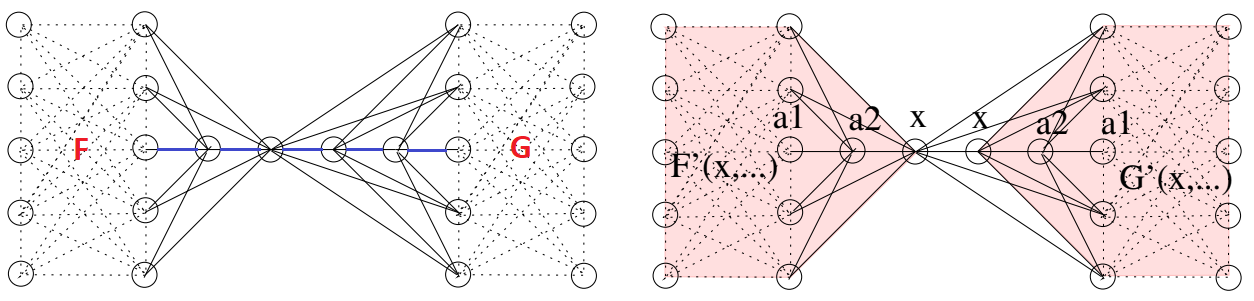
\includegraphics[width=\textwidth]{images/PostAlg.png}
	\caption{A graphical representation of the postprocessing algorithm involving two general penalty functions (F and G) linked by a chain (blue edges). It is important to notice the swap of role between the original node representing the shared variable to ensure consistency of the variable's value between functions.}
	\end{center}
\end{figure}
Post-processing cannot be applied to every quantum architecture. In order to be successful, it is necessary that qubits presents an high numbers of connections with other qubits. If this condition is not satisfied, we will not obtain great results from the re-computation of scores for penalty functions: nodes belonging to the chain will not link with external qubits and no new couplings to consider will emerge. D-Wave currently proposes two main architectures: the older one, Chimera, is clearly affected by this issue. Actually he graph of its nodes is sparse and a qubits has at most 6 neighbour qubits. On the other hand the most recent architecture, Pegasus, is less sparse and it usually does not fall into the issue described above. As a consequence, from now on we will assume that the algorithm will be executed only on the Pegasus architecture.


\section{Implementation}

While the definition of the approach is linear, in practice we have to deal with numerous issues, mainly caused by computational constraints. As a consequence, the implementation relies on some heuristic that avoid apparent deadlock point during execution.
The workflow of the implementation is shown in figure 4.2.
More details on each step will be provided in the next paragraphs.

\begin{figure}[t]
	\begin{center}
	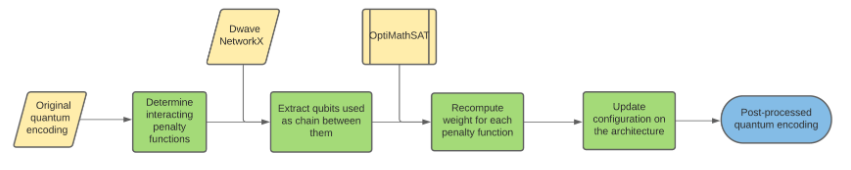
\includegraphics[width=\textwidth]{images/Workflow.png}
	\caption{A graphical representation of the workflow necessary to implement the postprocessing algorithm. Yellow nodes represent data and state-of-the-art tools; green nodes represent tasks implemented in this thesis.}
	\end{center}
\end{figure}

\subsection{Extracting encoding information}

The original version of the code returned the list of values assigned to each parameter, without any additional information about the mapping between Boolean sub-formulas and qubits. While it was not relevant in the precedent version, obtaining this information is now essential to determine how to rearrange qubits in new penalty functions. \\
To solve the issue, it was required to modify the \textit{place\_and\_route} library and collect data from the intermediate steps of the procedure. [Continue]

\subsection{Re-assigning qubits}

Once the needed data are stored and available, we can start to post-process the original encoding determining what functions might be extended and what chains are involved. For each pair of penalty functions we decide if there is a chain connecting them which can be split in two disjoint sub-sets of qubits without altering the correctness of the encoding of the original formula.

\subsection{Recomputing penalty functions}

In order to generate the OMT instance necessary to recompute the parameters on the enhanced penalty functions, we need to build the quadruplets of data necessary and call the \textit{searchPF} function using them.\\
We also tried to enhance the actual encoding, modifying the definition of the SMT file. 

\subsection{Updating the configuration}

\newpage


      \chapter{Results}
\label{cha:results}

\section{Ideal model}

\section{Application of CAIG17}

\newpage


      \chapter{Conclusions}
\label{cha:conclusioni}

In this thesis a novel approach to improve the definition of the SAT-to-Ising conversion has been heavily discussed. We have seen how the development of a postprocessing procedure can benefit the quantum encoding and provides more stable encodings. The most interesting success is represented by the capability of obtaining new penalty functions with higher minimum gaps simply re-arranging some qubits; this could guarantee an higher probability to search a final state satisfying the Boolean formula in the case. Albeit being still in a preliminary state, we have understood how this approach could lead to promising developments. We also proved how the average length of chains and the number of "wasted" chains drastically decrease when postprocessed, supporting the goal of trying to ov. \\
In addition to the postprocessing algorithm, the analysis of the old version of the tool put into evidence some minor issues that have led to further advancements. For instance, the extension of the Pegasus genlib file helped us in encoding more complex formulas using a more compact representation, reducing the number of chains and thus further stabilizing the resulting Hamiltonian problem. These aspects prove how the SAT-to-Ising problem is still in its primordial stages and there are considerable scope for improvements.

\section{Future work}

Even though a great deal of extensions and updates have been introduced, multiple ideas have aroused in the final stages, supporting the idea of new paths to follow to further improve the problem of SAT-to-Ising and related topics.

\subsection{Advancing SAT-to-Ising}

The first direction concentrates on expanding the current encoding algorithm and the postprocessing procedure. Some of these suggestions have been already mentioned in the previous chapters, in particular during the tool analysis. A list of possible challenges to address in the future concerns:

\begin{itemize}
    \item In the field of automated theorem proving and SMT, novel
techniques for solving quantified SMT formulas are emerging. It is thus possible to investigate these techniques for solving directly quantified formulas,
avoiding thus the expensive Shannon expansion which is applied when discussing equation 3.5.
    \item While Boolean function decomposition and minimization are mature classical subjects, those algorithms can probably be im-
proved by taking into consideration the specifics of the embedding (placement and routing onto a QA hardware graph) that follow them.
    \item Recently D-Wave announced the details of its next-generation computation hardware, which it is called "Advantage" and released a set of white papers that describe some of the machine's performance characteristics \cite{advantage}. The new architecture will have 5.000 qubits arranged in a 15x15x12 lattice. The number of couplings is drastically higher than Pegasus, with about 40000 connections. Lastly, D-Wave concentrated on lowering the noise of individual qubits, reaching a reduction by about three- to four-fold. Both the old algorithm and the postprocessing procedure should be tested on the new architecture, leading to better performances and offering cues for additional extensions.
\end{itemize}

\pagebreak

\subsection{Enhancing CP-to-OMT}

The second future direction to take into account focuses on bridging the gap between Constraint Programming and Optimization Modulo Theories. The open-source interface described in the previous chapters can be extended to efficiently manage each MiniZinc structure and procedure. To cover the full extent of CP standards some additions are required, such as defining an encoding based on Floating-Point Numbers or dealing with non-linear constraints and objectives. This may require a general review of the current implementation of the FlatZinc interface, so as to become modular and easy to extend.
Moreover, we can improve the situation by developing a T-solver for the theory of sets, which is currently managed using a quite inefficient mix of Boolean and arithmetic constraints. 
To conclude, another interesting issue concerns CP global constraints, constraints that capture a relation between a non-fixed number of variables. In particular, it would be necessary to study approaches to integrate dedicated procedures to the SMT and OMT framework emulating these constraints. \\
 





      
    \endgroup


    % bibliografia in formato bibtex
    %
    % aggiunta del capitolo nell'indice
    \addcontentsline{toc}{chapter}{Bibliografia}
    % stile con ordinamento alfabetico in funzione degli autori
    \bibliographystyle{plain}
    \bibliography{biblio}
%%%%%%%%%%%%%%%%%%%%%%%%%%%%%%%%%%%%%%%%%%%%%%%%%%%%%%%%%%%%%%%%%%%%%%%%%%
%%%%%%%%%%%%%%%%%%%%%%%%%%%%%%%%%%%%%%%%%%%%%%%%%%%%%%%%%%%%%%%%%%%%%%%%%%
%% Nota
%%%%%%%%%%%%%%%%%%%%%%%%%%%%%%%%%%%%%%%%%%%%%%%%%%%%%%%%%%%%%%%%%%%%%%%%%%
%% Nella bibliografia devono essere riportati tutte le fonti consultate 
%% per lo svolgimento della tesi. La bibliografia deve essere redatta 
%% in ordine alfabetico sul cognome del primo autore. 
%% 
%% La forma della citazione bibliografica va inserita secondo la fonte utilizzata:
%% 
%% LIBRI
%% Cognome e iniziale del nome autore/autori, la data di edizione, titolo, casa editrice, eventuale numero dell’edizione. 
%% 
%% ARTICOLI DI RIVISTA
%% Cognome e iniziale del nome autore/autori, titolo articolo, titolo rivista, volume, numero, numero di pagine.
%% 
%% ARTICOLI DI CONFERENZA
%% Cognome e iniziale del nome autore/autori (anno), titolo articolo, titolo conferenza, luogo della conferenza (città e paese), date della conferenza, numero di pagine. 
%% 
%% SITOGRAFIA
%% La sitografia contiene un elenco di indirizzi Web consultati e disposti in ordine alfabetico. 
%% E’ necessario:
%%   Copiare la URL (l’indirizzo web) specifica della pagina consultata
%%   Se disponibile, indicare il cognome e nome dell’autore, il titolo ed eventuale sottotitolo del testo
%%   Se disponibile, inserire la data di ultima consultazione della risorsa (gg/mm/aaaa).    
%%%%%%%%%%%%%%%%%%%%%%%%%%%%%%%%%%%%%%%%%%%%%%%%%%%%%%%%%%%%%%%%%%%%%%%%%%
%%%%%%%%%%%%%%%%%%%%%%%%%%%%%%%%%%%%%%%%%%%%%%%%%%%%%%%%%%%%%%%%%%%%%%%%%%
    

    \titleformat{\chapter}
        {\normalfont\Huge\bfseries}{Allegato \thechapter}{1em}{}
    % sezione Allegati - opzionale

\end{document}
